\chapter{Interacción Débil}\label{cap:weak_int}
El origen de cada interacción fundamental se debe a causas diferentes. Por un lado, la existencia de carga eléctrica produce fuerzas electromagnéticas en las partículas y las hace interactuar entre sí, mientras que la interacción fuerte se debe a la propiedad del color, mencionada en el capítulo anterior. No todas las partículas tienen carga ni color simultáneamente por lo que no todas son susceptibles a las mismas interacciones. El caso de la interacción débil es bastante interesante porque muchas partículas con propiedades distintas son sensibles a ella. Por ejemplo, los leptones no tienen carga de color, no ``sienten'' la interacción fuerte, mientras los neutrinos no tienen carga eléctrica, por lo que no pueden interactuar mediante fuerzas electromagnéticas. Sin embargo, ambos tipos de partículas pueden estar presentes en interacciones débiles \cite{Griffiths2008}. Además, la causa de la interacción débil, aunque no tiene un nombre específico, suele denotarse como \textit{carga débil}.

Los mesones $\PK$ y muchas otras partículas decaen por interacción débil. Desde el principio se consideró un tratamiento cuántico-relativista para describir la fuerza débil y muchos científicos han contribuido al desarrollo de su formalismo. Cada interacción ocurre gracias al intercambio de una partícula mediadora o portadora de la fuerza de interacción. En la interacción fuerte es el gluón y en la electromagnética es el fotón. Las partículas mediadoras encargadas de transmitir la fuerza débil entre los quarks y leptones son los bosones vectoriales, llamados así por tener espín 1. Estos bosones, de gran masa, portadores de la interacción débil pueden estar cargados eléctricamente $\PWpm$ o ser neutros $\PZzero$. 

Hasta la década de los 70, sólo se habían observado procesos de intercambio de bosones cargados $\PWpm$. En los años 60 se empezó a formular una teoría que aunaba la interacción débil junto con la electromagnética, conocida hoy en día como \textit{Teoría Electrodébil}. Esta teoría predecía la existencia del bosón neutro mediador de la fuerza débil y dicha hipótesis fue confirmada experimentalmente en 1973 \cite{BrianM}, con el hallazgo de $\PZzero$.

Este capítulo se centra, principalmente, en la descripción de procesos de interacción débil con intercambio de bosones $\PWpm$ o procesos de \textit{interacción débil de corriente cargada} y nos servirá como base para el estudio del decaimiento de mesones $\PK$ cargados.

\section{Formalismo de la Interacción Débil}\label{cap:formalism}
La interacción débil se postula de forma análoga a la interacción electromagnética, la cual se basa en el acoplamiento del fotón con las corrientes electromagnéticas debidas a las cargas eléctricas en las partículas. Así, para la fuerza débil, se tienen corrientes débiles que se acoplan a los bosones vectoriales $\PWpm$ o $\PZzero$. De acuerdo con la Teoría Cuántica de Campos (TCC), cada partícula lleva asociado un campo cuántico $\phi(x)$, $\psi(x)$ o $W_{\mu}(x)$, dependiente del espacio y del tiempo $x^{\mu}=(ct,\boldsymbol{\vec{x}})$\protect\footnotemark. Estos campos actúan como operadores encargados de aniquilar partículas o crear antipartículas de espín $0$, $1/2 $ y $1$, respectivamente \cite{notas2020}. Para describir la evolución espacio-temporal de dichos campos asociados a partículas se hace uso de la densidad lagrangiana $\mathcal{L}$.

\footnotetext{Consultar el Apéndice \hyperref[cap:A]{A} para más información sobre la notación utilizada en este capítulo.}

Del mismo modo, las interacciones se describen mediante unas constantes, denominadas \textit{contantes de acoplamiento}, y productos entre los campos cuánticos de las partículas que intervienen en el proceso. Como $\mathcal{L}$ debe ser un escalar, sólo se permiten combinaciones entre campos que resulten en invariantes de Lorentz \cite{notas2020}. Esto es posible, ya que la TCC, entiende las interacciones como un intercambio de partículas mediadoras, tal y como se mencionó anteriormente. En su libro \cite{Bettini}, Bettini lo explica con el siguiente ejemplo: se tiene una partícula $a$ que interactúa en el campo mediado por el bosón $V$; en el vacío, $a$ está continuamente emitiendo y absorbiendo este bosón, tal y como se muestra en \ref{fig:bettini1}. No obstante, si una partícula $b$ se encuentra cerca de $a$ y tiene su misma interacción, puede absorber un bosón $V$ que previamente haya sido emitido por $a$ (ver \ref{fig:bettini2}). Entonces, se puede afirmar que $a$ y $b$ interactúan entre sí intercambiando un bosón $V$, es decir, combinando sus campos cuánticos mientras se crea y se aniquila $V$.
\begin{figure}[h]
\begin{subfigure}{.5\textwidth}
  \centering
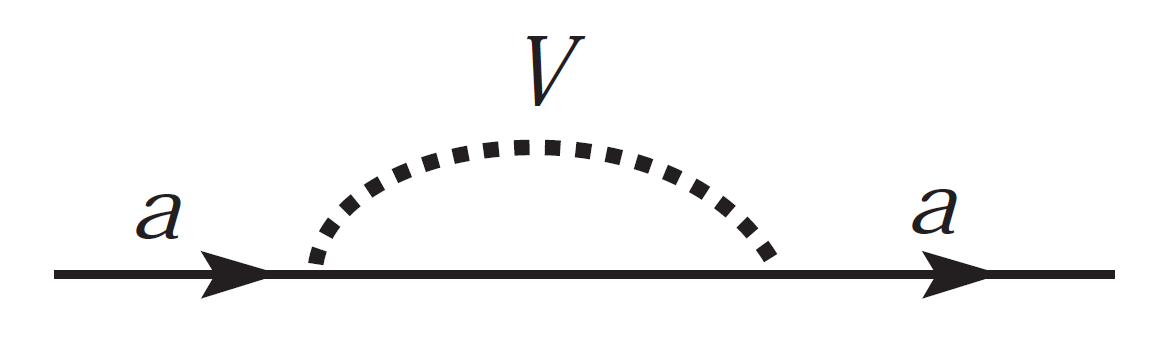
\includegraphics[width=0.6\linewidth]{{C:/Users/Carmen/Desktop/Universidad/TFG/Borradores/img/bettini1.PNG}}
\caption{$V$ emitido y reabsorbido por $a$}
  \label{fig:bettini1}
\end{subfigure}%
\begin{subfigure}{.5\textwidth}
  \centering
  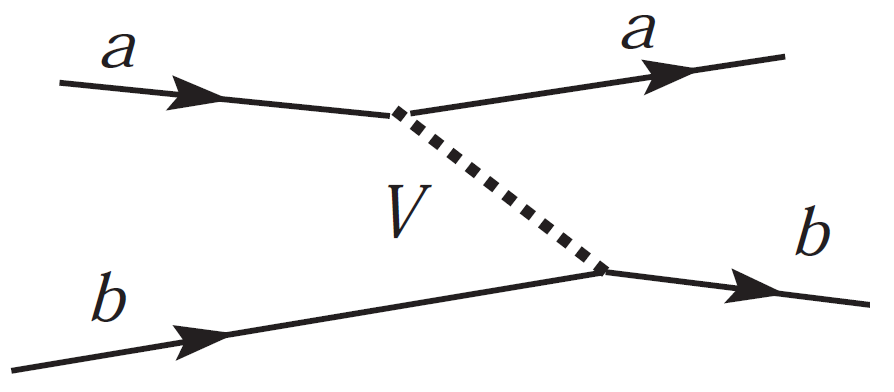
\includegraphics[width=0.6\linewidth]{{C:/Users/Carmen/Desktop/Universidad/TFG/Borradores/img/bettini2.PNG}}
  \caption{$V$ emitido por $a$ y absorbido por $b$}
  \label{fig:bettini2}
\end{subfigure}
\caption[Esquematización del proceso de interacción en TCC]{Proceso de interacción mediante intercambio del bosón mediador.  \cite{Bettini}}
\label{fig:bettini}
\end{figure}

Continuando con el ejemplo anterior, Bettini indica que el bosón mediador $V$ tiene, en general, una masa $m$ no nula, lo que provoca que, durante su emisión, se viole momentáneamente la conservación de energía $\Delta E = m$. Lo mismo, pero de forma opuesta ocurre durante su absorción. Así pues, la violación neta dura un $\Delta t$ y satisface la \textit{Relación de Indeterminación tiempo-energía}: $\Delta E \Delta t \leq \hbar$, lo que implica que $V$ sólo puede alejarse una distancia finita $R=c\Delta t$. Esta distancia equivale al rango de la fuerza de interacción, por lo tanto, cuanta mayor masa tenga el bosón mediador de una interacción, menor será su rango de alcance \cite{Bettini}. Dado que los bosones mediadores $\PWpm$ y $\PZzero$ tienen una masa muy grande ($m_W = \SI{80,379 \pm 0,012}{\GeV}$ y $m_Z = \SI{91,1876 \pm 0,0021}{\GeV}$, respectivamente \cite{Zyla}), la fuerza débil tiene un alcance muy corto, más que cualquier otra interacción fundamental, resultando en una intensidad muy tenue; de ahí la denominación de ``interacción débil''. 

Gráficamente, las interacciones se representan con Diagramas de Feynman. Estos diagramas proporcionan información acerca de la amplitud de probabilidad de los distintos procesos, donde cada línea representa a una partícula y cada vértice corresponde a cada actuación del lagrangiano de la interacción $\mathcal{L}$. La densidad lagrangiana $\mathcal{L}$ que describe cada vértice en el Diagrama de Feynman de una interacción de corriente cargada débil, tiene esta forma:
\begin{equation}
\mathcal{L}^{w}=\dfrac{g_{w}}{\sqrt{2}}\left( W^{\mu }\left( x\right) j_{\mu}^{+}\left( x\right) +\left[ W^{\mu }\left( x\right) \right]^{\ast }j_{\mu}^{-}\left( x\right) \right)\label{eq:weak_lagrangian}
\end{equation}

El campo $W^{\mu}(x)$ aniquila $\PWp$ o crea $\PWm$ mientras que su conjugado $\left(W^{\mu}(x)\right)^\ast$ aniquila $\PWm$ o crea $\PWp$. En un proceso que ocurre por interacción débil con intercambio de $\PWpm$, la carga neta del estado inicial y el final difieren en una unidad y, entonces, se habla de interacción de corriente cargada. Luego, la densidad de corriente débil $j_{\mu}$ puede ser positiva o negativa, y se compone de dos términos, uno para la corriente leptónica y otro para la hadrónica:
\begin{equation}
j_{\mu} ^{\pm }\left( x\right) =j_{\mu} ^{\pm lep}\left( x\right) +j_{\mu} ^{\pm had}\left( x\right) \label{eq:weak_current_hadylep}
\end{equation}
La corriente leptónica es una composición de corrientes de cada familia de leptones, así se tiene un término para los electrones, otro para los muones y otro para los taones:
\begin{equation}
j_{\mu }^{\pm lep}\left( x\right) =j_{\mu }^{\pm el}\left( x\right) +j_{\mu }^{\pm muon}\left( x\right) +j_{\mu} ^{\pm tau}\left( x\right)\label{eq:leptonic_weak_current}
\end{equation}
La corriente leptónica de electrones puede expresarse de la siguiente forma:
\begin{align}
j_{\mu }^{-el}\left(x\right)&=i\overline{\psi}_{e}\left( x\right) \dfrac{1-\gamma_{5}}{2}\gamma _{\mu }\psi_{{ \nu}_{e}}\left( x\right) & j_{\mu}^{+el}\left(x\right)&= i\overline{\psi}_{{\nu}_{e}}\left(x\right) \dfrac{1-\gamma_{5}}{2}\gamma _{\mu}\psi_{e}\left( x\right)\label{eq:electric_weak_current}
\end{align}
La corriente negativa $j_{\mu }^{-el}$, aniquila $\nu_e$ (o crea $\overline{\nu_e}$) y crea $e^-$ (o aniquila $e^+$), mientras que la corriente positiva $j_{\mu }^{+el}$ hace justo lo opuesto. $j_{\mu }^{\pm muon}$ y $j_{\mu }^{\pm tau}$ pueden definirse de manera análoga. Estas corrientes leptónicas se caracterizan por conservar el número cuántico leptónico y la carga de las partículas que intervienen. 

El operador de corriente hadrónica $j_{\mu} ^{\pm had}$ es el encargado de crear o aniquilar hadrones, conservando siempre el número bariónico $B$ e incrementando o reduciendo en una unidad la carga eléctrica total $Q$. Sin embargo, aunque no siempre, también son capaces de modificar la extrañeza: la corriente hadrónica positiva (negativa) puede aumentar (disminuir) la extrañeza en una unidad $\Delta S = +1$ ($\Delta S = -1$) \cite{notas2020}.

Además, $g_W$ es la constante de acoplo de la interacción débil y se relaciona con la constante de Fermi $G_F$ según \ref{eq:fermi_coupling}. Experimentalmente se ha comprobado que $G_F$ tiene un valor único para todos los procesos donde interviene la interacción débil, siendo este $G_{F}= \SI{1,166e-5}{\per\GeV\squared}$.
\begin{equation}
\dfrac{G_{F}}{{g_{w}}^2}=\dfrac{\sqrt{2}}{8{m_{W}}^2}\label{eq:fermi_coupling}
\end{equation}

Si se reescribe la corriente débil leptónica de la ecuación \ref{eq:electric_weak_current} en su forma expandida, pueden distinguirse dos términos:
\begin{equation}
j_{\mu}^{+el}\left(x\right)= \dfrac{i}{2} \{ \overline{\psi}_{{\nu}_{e}}\left(x\right)\gamma _{\mu}\psi_{e}\left( x\right)- \overline{\psi}_{{\nu}_{e}}\left(x\right)\gamma _{\mu}\gamma_{5}\psi_{e}\left( x\right) \}
\end{equation}
El primero $\overline{\psi}_{{\nu}_{e}}\gamma _{\mu}\psi_{e}$ se transforma como un vector polar (V) y el segundo término $\overline{\psi}_{{\nu}_{e}}\gamma _{\mu}\gamma_{5}\psi_{e}$ como un vector axial (A). Debido a esto, la corriente débil se dice que tiene estructura V-A. Esta estructura no es exclusiva para la corriente débil leptónica, sino que también está presente en la corriente débil hadrónica, salvo alguna constante de acoplamiento. 

Inicialmente, se introdujo la parte correspondiente al vector polar en la corriente débil por analogía con la interacción electromagnética. El término del vector axial fue añadido posteriormente, tras el descubrimiento de la violación de paridad \cite{Paschos}. Si una interacción presenta la estructura anterior de Vector polar - vector Axial, se dice que es una \textit{Interacción V-A}.

Por lo tanto, el lagrangiano $\mathcal{L}$ de una interacción débil presentar estructura V-A o, en su forma más general, una combinación o producto de estructuras V-A \cite{Renton}, una para describir el decaimiento de los leptones y otra para los quarks:
\begin{equation}
\mathcal{L}= \sum _{i} C_{i}\left(\overline{\psi}_{\nu_l}\widehat{\Gamma_{i}}\psi _{l}\right)\left( \overline{\psi }_{q_2}\widehat{\Gamma^{i}}\psi _{q_1}\right)
\end{equation}
Los coeficientes $C_i$ son constantes de acoplamiento del proceso en cuestión y los $\psi_i$ son los bi-espinores resultantes de la ecuación de Dirac que describe cada fermión (quark o lepton) que participa en la interacción. Los $\widehat{\Gamma_{i}}$ son covariantes bilineales, los cuales proporcionan información sobre cómo se transforman dichas partículas (ver Apéndice \hyperref[cap:A]{A}).

A la hora de analizar el decaimiento de mesones $\PK$, la magnitud que más interesa calcular es la probabilidad de decaimiento $\Gamma$. $\Gamma$ indica la probabilidad por unidad de tiempo de que el kaón (o cualquier partícula) sufra un proceso de desintegración. Por ejemplo, si se tiene un conjunto de partículas $N(t)$ en un instante $t$, una porción $N\Gamma dt$ de ellas decaerá en el próximo instante $dt$ \cite{Griffiths2008}:
\begin{align}
dN &= -\Gamma Ndt & N(t) &= N(0)e^{-\Gamma t}
\end{align}
Además, esta magnitud $\Gamma$ está relacionada con la semivida de la partícula $\tau$:
\begin{equation}
\tau=\dfrac{1}{\Gamma}\label{eq:meanlife}
\end{equation}
Como, en general, las partículas pueden decaer de distintas formas o modos:
\begin{align}
\Gamma_{total} &= \sum_{i=1}^N \Gamma_i & \tau=\dfrac{1}{\Gamma_{total}}
\end{align}
Por este motivo, también es posible definir el ratio de desintegración o branching ratio ($BR$) para un modo de decaimiento $i$ dado:
\begin{equation}
BR(i)=\dfrac{\Gamma_{i}}{\Gamma_{total}}
\end{equation}

En unidades naturales ($\hbar=c=1$), la probabilidad de decaimiento $\Gamma$ es:
\begin{equation}
2\pi \left| \mathcal{M}\right| ^{2} \rho\left( E\right)
\end{equation} 
Siendo $\mathcal{M}$ la amplitud de probabilidad y $\rho\left(E\right) \equiv \rho$ la densidad de estados finales del proceso.

Por un lado, la densidad de estados finales (o espacio de fases) depende de las masas, las energías y los momentos de las partículas que intervienen en el decaimiento, es decir, contiene toda la información cinemática del proceso. Por otra parte, la amplitud de probabilidad (también conocida como elemento de matriz) es una magnitud que está relacionada con el lagrangiano de la interacción $\mathcal{L}$ y, por lo tanto, proporciona información acerca de la dinámica del decaimiento. 

Los mesones $\PK$ son partículas de espín 0, por lo que el campo escalar que los describe satisface la ecuación de Klein-Gordon, que en forma covariante tiene la siguiente expresión:
\begin{equation}
\left( \square +m^{2}\right) \psi \left( x\right) =0
\end{equation}

Además, la densidad lagrangiana ${\mathcal{L}}^w$ que describe el decaimiento de los mesones $\PK$ por interacción débil es invariante de Lorentz, por lo que se cumple que \cite{Halzen}
\begin{equation}
\mathcal{M}=-i \int {\mathcal{L}}^w \left(x\right) d^{4}x \propto -i\int j_{\mu }W^{\mu }d^{4}x
\end{equation}

Para hallar $d\Gamma$, se hace uso de la \textit{Regla de Oro de Fermi} para procesos de desintegración del tipo $1 \rightarrow 2+3$:
\begin{equation}
d\Gamma =\left| \mathcal{M}\right| ^{2}\dfrac{S}{2m_{1}}\left[ \left( \dfrac{d^{3}\boldsymbol{p}_{2}}{\left( 2\pi \right) ^{3}2E_{2}}\right) \left( \dfrac{d^{3}\boldsymbol{p}_{3}}{\left( 2\pi \right) ^{3}2E_{3}}\right) \right] \times \left( 2\pi \right) ^{4}\delta ^{4}\left( p_{1}-p_{2}-p_{3}\right) 
\end{equation}

Los diagramas de Feynman son una herramienta muy útil a la hora de calcular de forma rápida y sencilla $\left| \mathcal{M}\right|$. Para ello, sólo debemos de seguir las reglas del cálculo de Feynman en unidades naturales \cite{Griffiths2008}:

\begin{enumerate}
\item \underline{Notación}: Etiquetar todos los cuadri-momentos (internos y externos) del proceso y asignar flechas a cada línea.
\item \underline{Líneas externas}: Para partículas y antipartículas llegando al vértice escribir los espinores $u$ y $\overline{v}$, respectivamente. Si salen del vértice, entonces se escribe: $\overline{u}$ y $v$, en cada caso.
\item \underline{Factor de vértice}: Para cada vértice, escribir un factor $\dfrac{-ig_{w}}{2\sqrt{2}}\gamma ^{\mu }\left( 1-\gamma ^{5}\right)$. 
\item \underline{Propagadores}: Para cada línea interna que represente un bosón vectorial $\PWpm$ o $\PZzero$, escribir un factor: 
$\dfrac{-i\left( g_{\mu\nu }-q_{\mu }q_{\nu }/M^{2}\right) }{q^{2}-M^{2}}$. Pero, en general, como $q^{2}\ll \left( M\right)^{2}$ puede realizarse la siguiente aproximación para describir el vértice: $\dfrac{ig_{\mu \nu }}{\left( M\right) ^{2}}$.
\item \underline{Conservación de momento y energía}: Para cada vértice, escribir $\left( 2\pi \right) ^{4}\delta ^{4}\left( k_{1}+k_{2}+k_{3}\right)$. En esta expresión $k$ es el vector momento de 3 componentes dirigiéndose hacia el vértice. Si el momento sale del vértice entonces lleva un signo menos.
\item \underline{Integrar sobre todos los momentos}: Para cada cuadri-momento $q$, escribir un factor $\dfrac{d^{4}q}{\left( 2\pi \right) ^{4}}$ e integrar.
\item \underline{Cancelar la función Delta $\Delta$}: Cancelar el factor restante $\left( 2\pi \right) ^{4}\delta ^{4}\left( p_{1}+p_{2}+\ldots -p_{n}\right)$ e igualar la expresión resultante a $-i\mathcal{M}$.
\end{enumerate}


\subsection{Interacción débil en el Modelo de Quarks}\label{sec:weak_int_quarks}
En el modelo de Quarks, la interacción débil se describe mediante Diagramas de Feynman, donde se produce un cambio de sabor en los quarks, emitiendo bosones $\PWpm$. Como consecuencia de la conservación del número leptónico en esta interacción, el acoplamiento de $\PWpm$ ocurre de manera estricta entre leptones de la misma generación \cite{Griffiths2008}: 
\begin{align}
\begingroup 
\renewcommand*{\arraystretch}{0.8}
\setlength\arraycolsep{10pt}
\begin{pmatrix} \nu _{e} \\ e \end{pmatrix} \qquad
\begin{pmatrix} \nu_{\mu } \\ \mu \end{pmatrix} \qquad
\begin{pmatrix} \nu_{\tau} \\ \tau \end{pmatrix}
\endgroup
\end{align}
No obstante, $W^{\pm}$ sí puede acoplarse a quarks de distintas generaciones:
\begin{align}
\begingroup 
\renewcommand*{\arraystretch}{0.8}
\setlength\arraycolsep{10pt}
\begin{pmatrix} u \\ d \end{pmatrix} \qquad
\begin{pmatrix} c \\ s \end{pmatrix} \qquad
\begin{pmatrix} t \\ b \end{pmatrix}
\endgroup
\end{align}

Cuando únicamente se habían descubierto los quarks ligeros, en torno a 1963, Cabibbo sugirió que este acoplamiento inter-generacional como explicación al fenómeno de violación de la extrañeza en la interacción débil. Así, en un Diagrama de Feynman, la corriente hadrónica débil mantiene la estructura V-A, pero su expresión puede variar dependiendo de si se conserva o no la extrañeza en el vértice a estudio del proceso:
\begin{itemize}
\item Sin cambio de extrañeza, se aniquila un quark $\Pqd$ y se crea un quark $\Pqu$: $\Pqd \rightarrow \Pqu + \PWm$
\end{itemize}
\begin{equation}
j_{\mu}^{+had}(\Delta S= 0)=\cos \left( \theta _{c}\right) i\overline{\psi }_{u}\left( x\right) \dfrac{1-\gamma _{5}}{2}\gamma _{\mu }\psi _{d}
\end{equation}
\begin{itemize}
\item Con cambio de extrañeza, se aniquila un quark $s$ y se crea un quark $\Pqu$: $\Pqs \rightarrow \Pqu + \PWm$
\end{itemize}
\begin{equation}
j_{\mu}^{+had}(\Delta S= 0)=\sin \left( \theta _{C}\right) i\overline{\psi }_{u}\left( x\right) \dfrac{1-\gamma _{5}}{2}\gamma _{\mu }\psi _{s}
\end{equation}
donde $\theta_{C}$ hace referencia al ángulo de Cabibbo, cuyo valor experimental ha resultado ser $13,02\degree$.

La teoría de Cabibbo era bastante acertada al dar explicación a numerosos decaimientos de quarks. Sin embargo, esta teoría también permitía el decaimiento del mesón $\PKz$ en $\APmuon\Pmuon$, cuya amplitud de probabilidad era proporcional a $\cos \left( \theta _{C}\right) \sin \left( \theta _{C}\right)$ y, por lo tanto, mucho mayor que la obtenida experimentalmente.  Para solucionar esta contradicción, en 1970, Glashow, Iliopoulos y Maiani (GIM), propusieron la existencia de un nuevo quark $\Pqc$ que debía acoplarse con $-\Pqd \cdot \sin \left( \theta _{C}\right) + \Pqs \cdot \cos \left( \theta_C \right)$, la combinación ortogonal a $\Pqd \cdot \cos \left( \theta _{C}\right) + \Pqs \cdot \sin \left( \theta _{C}\right)$, a la que se acoplaba el sabor $\Pqu$ \cite{Griffiths2008}.

Nacía así, la teoría Cabibbo-GIM, la cual afirmaba que los estados de los quarks $\Pqd$ y $\Pqs$, en lugar de su descripción física, debían definirse como:
\begin{equation}
\begin{gathered}
\Pqd'=\Pqd \cdot \cos \left( \theta _{C}\right) + \Pqs \cdot \sin \left( \theta _{C}\right) \\
\Pqs'= - \Pqd \cdot \sin \left( \theta _{C}\right) + \Pqs \cdot \cos \left( \theta_C\right)
\end{gathered}
\end{equation}
De manera que los $\PWpm$ se acoplaran a las familias de quarks como hacían los leptones, pero con la definición correcta de los estados de los quarks o quarks \textit{rotados}:
\begin{align}
\begingroup 
\renewcommand*{\arraystretch}{0.8}
\setlength\arraycolsep{10pt}
\begin{pmatrix} \Pqu \\ \Pqd' \end{pmatrix} \qquad
\begin{pmatrix} \Pqc \\ \Pqs' \end{pmatrix}
\endgroup
\end{align}

En 1973, Kobayashi y Maskawa, en un intento de dar explicación a la violación CP, generalizaron el esquema de Cabibbo-GIM, para incluir una tercera generación de quarks, aún sin descubrir en aquel entonces, surgiendo así la \textit{matriz CKM} (Cabibbo-Kobayashi-Maskawa):
\begin{equation}
\begingroup 
\renewcommand*{\arraystretch}{0.8}
\setlength\arraycolsep{10pt}
\begin{pmatrix} \Pqd' \\ \Pqs' \\ \Pqb' \end{pmatrix} =\begin{pmatrix} V_{ud} & V_{us} & V_{ub} \\ V_{cd} & V_{cs} & V_{cb} \\ V_{td} & V_{ts} & V_{tb} \end{pmatrix}\begin{pmatrix} d \\ s \\ b \end{pmatrix}
\endgroup\label{eq:CKM}
\end{equation}

Esta matriz permitía conectar todos los sabores de quarks entre sí, siendo los elementos de su diagonal los más importantes, al relacionar quarks de la misma familia: $\Pqu \leftrightarrow \Pqd$, $\Pqc \leftrightarrow \Pqs$ y $\Pqt \leftrightarrow \Pqb$. En definitiva, proporciona información acerca de la probabilidad de transición de un quark $i$ a un quark $j$. Los términos no diagonales son los responsables de que los quarks pesados vayan decayendo progresivamente en los sabores ligeros $\Pqu$ y $\Pqd$, que son los constituyentes predominantes de la materia ordinaria. Así, por ejemplo, $V_{ud}$ describe el acoplamiento de $\Pqu$ a $\Pqd$: $\Pqd \rightarrow \Pqu + \PWm$.

La matriz CKM puede reducirse a una especie de ``forma canónica'' utilizando los \textit{ángulos generalizados de Cabibbo} $\theta_{1}$, $\theta_{2}$, $\theta_{3}$, y un factor de fase $e^{i\delta}$ \cite{Griffiths2008}:
\begin{equation}
\begingroup 
\renewcommand*{\arraystretch}{0.8}
\setlength\arraycolsep{10pt}
|V|=
\begin{pmatrix} c_{1} & s_{1}c_{3} & s_{1}s_{3} \\ -s_{1}c_{2} & c_{1}c_{2}c_{3}-s_{2}s_{3}e^{i\delta } & c_{1}c_{2}s_{3}+s_{2}c_{3}e^{i\delta } \\ -s_{1}s_{2} & c_{1}s_{2}c_{3}+c_{2}s_{3}e^{i\delta } & c_{1}s_{2}s_{3}-c_{2}c_{3}e^{i\delta } \end{pmatrix}
\endgroup
\end{equation}

con $c_{i}\equiv \cos \theta _{i}$ y $s_{i}\equiv \sin \theta _{i}$.

Si $\theta _{2}=\theta _{3}=0$, entonces $\theta _{1}=\theta _{C}$, obteniéndose la representación Cabibbo-GIM anterior. Los elementos $|V_{ij}|$ de la matriz CKM suelen determinarse empíricamente, pero en concreto, el promedio de $|V_{ud}|$ y el de $|V_{us}|$ se conocen con bastante exactitud.\\

\section{Decaimiento de mesones $K$ cargados}
\label{sec:charged_kaon_decay}
Los mesones $\PKpm$ decaen por interacción débil y sus procesos de decaimiento (modos) pueden clasificarse en varias categorías. A continuación, presentamos los modos leptónicos, semileptónicos y hadrónicos, que son los más relevantes:

\begin{table}[!htb]
\begin{minipage}{.5\linewidth}
    \centering
\begin{tabular}{ c c } 
\toprule
\makecell{Mesón $\PKp$}  &  Mesón $\PKm$ \\
\midrule   
$\Pep\Pnu_{e}$ & $\Pem\APnu_{e}$ \\
$\APmuon\Pnu_{\mu}$ & $\Pmuon\APnu_{\mu}$ \\
$\Pgpz\Pep\Pnu_{e}$ & $\Pgpz\Pem\APnu_{e}$ \\
$\Pgpz\APmuon\Pnu_{\mu}$ & $\Pgpz\Pmuon\APnu_{\mu}$ \\
$\Pgpz\Pgpz\Pep\Pnu_{e}$ & $\Pgpz\Pgpz\Pem\APnu_{e}$ \\
$\Pgpp\Pgpm\Pep\Pnu_{e}$ & $\Pgpp\Pgpm\Pem\APnu_{e}$ \\
$\Pgpp\Pgpm\APmuon\Pnu_{\mu}$ & $\Pgpp\Pgpm\Pmuon\APnu_{\mu}$ \\
$\Pgpz\Pgpz\Pgpz\Pep\Pnu_{e}$ & $\Pgpz\Pgpz\Pgpz \Pem \APnu_{e}$ \\
\bottomrule
\end{tabular}
\caption[Modos de decaimiento leptónicos y semileptónicos de $\PKpm$]{Modos (semi-)leptónicos. \cite{Zyla}}
\label{tab:Kpm_leptonic_decay}
\end{minipage}\hfill
\begin{minipage}{.5\linewidth}
    \centering
\begin{tabular}{ c c } 
    \toprule
    \makecell{Mesón $\PKp$}  &  Mesón $\PKm$ \\    
    \midrule
$\Pgpp\Pgpz$ & $\Pgpm\Pgpz$ \\
$\Pgpp\Pgpz\Pgpz$ & $\Pgpm\Pgpz\Pgpz$ \\
$\Pgpp\Pgpp\Pgpm$ & $\Pgpp\Pgpm\Pgpm$ \\
    \bottomrule
\end{tabular}
\caption[Modos de decaimiento hadrónicos de $\PKpm$]{Modos hadrónicos. \cite{Zyla}}
\label{tab:Kpm_hadronic_decay}
\end{minipage}
\end{table}

Como puede observarse, los modos de decaimiento de $\PKm$ son los mismos modos que los de $\PKp$ pero con carga conjugada. Sin embargo, no todos estos procesos tienen la misma probabilidad de ocurrir. Como ejemplo ilustrativo de esta afirmación, centramos el estudio en los modos leptónicos del mesón $\PKm$: $\PKm \rightarrow \Pem \APnu_{e}$ y $\PKm \rightarrow \Pmuon \APnu_{\mu}$.

El Diagrama de Feynman de quarks de $\PKm \rightarrow \Plm + \Pagnl$ aparece en la figura \ref{fig:diagrama1}.

\begin{figure}[ht!]
	\centering
	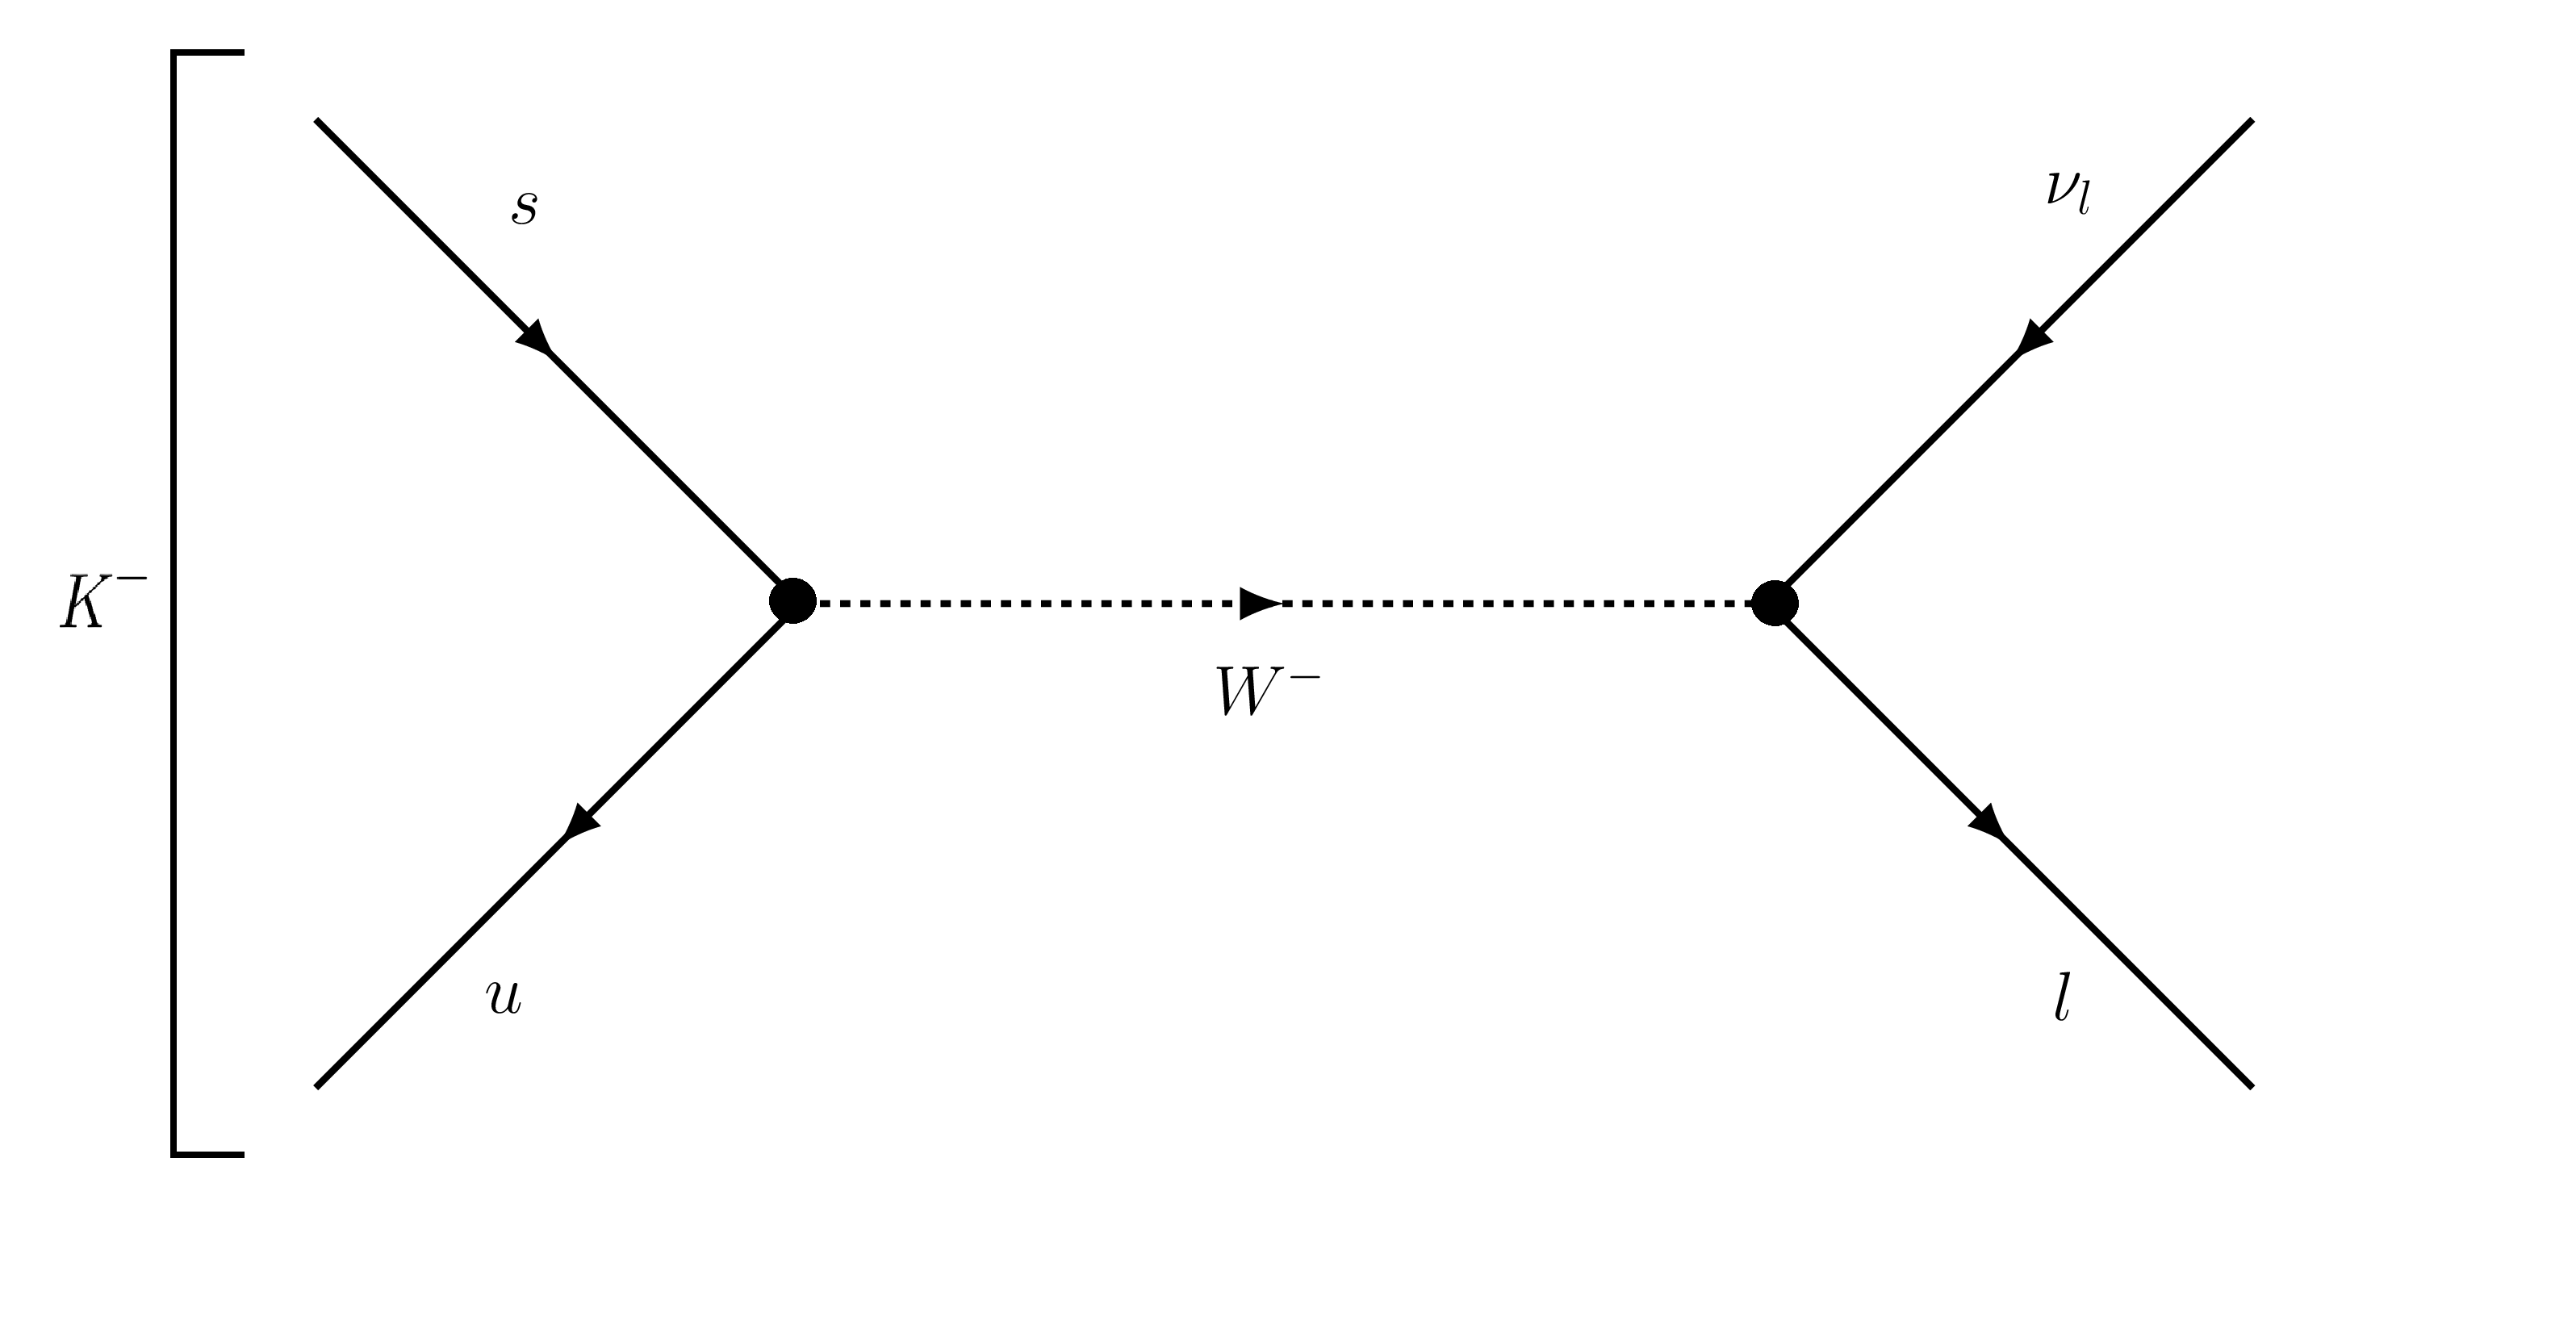
\includegraphics[width=0.95\textwidth]{C:/Users/Carmen/Desktop/Universidad/TFG/Borradores/img/kaon1.png}
	\caption[Diagrama de Feynman de quarks de $\PKm \rightarrow \Plm + \Pagnl$]
	{Diagrama de Feynman del modo leptónico de $\PKm$ en el Modelo de Quarks.}
	\label{fig:diagrama1}
\end{figure}

El vértice leptónico está totalmente definido a partir de las expresiones de corriente débil vistas en el formalismo anterior. Sin embargo, el vértice hadrónico es algo más complejo de explicar y puede hacerse mediante dos enfoques. El primero de ellos consiste en una descripción a partir de la composición de quarks de $\PKm$, pero este tratamiento presenta una dificultad de cálculo y formalismo teórico demasiado avanzado. Por ello, y dado que el mesón $\PK$ es una partícula de espín 0, resulta más sencillo describir dicho vértice hadrónico a partir de la ecuación de Klein-Gordon.

Siguiendo este segundo procedimiento, redibujamos el diagrama $\PKm \rightarrow \Plm + \Pagnl$ como se ve en la figura \ref{fig:diagrama2}, donde también se han etiquetado los momentos internos y externos de cada partícula que interviene. El punto gordo que se aprecia en el vértice hadrónico, simplemente indica que, como el mesón $\PKm$ posee una estructura interna más elemental de quarks, no sabemos de antemano cómo interacciona con el propagador $\PWm$. Por ello, para el vértice hadrónico se escribe un factor: $\dfrac{-ig_{w}}{2\sqrt{2}}F^{\mu}$. El término $F^{\mu}$ se conoce como \textit{factor de forma}; es un cuadrivector dependiente del momento del mesón $\PKm$ que describe la interacción en el vértice hadrónico con el propagador.

\begin{figure}[ht!]
	\centering
	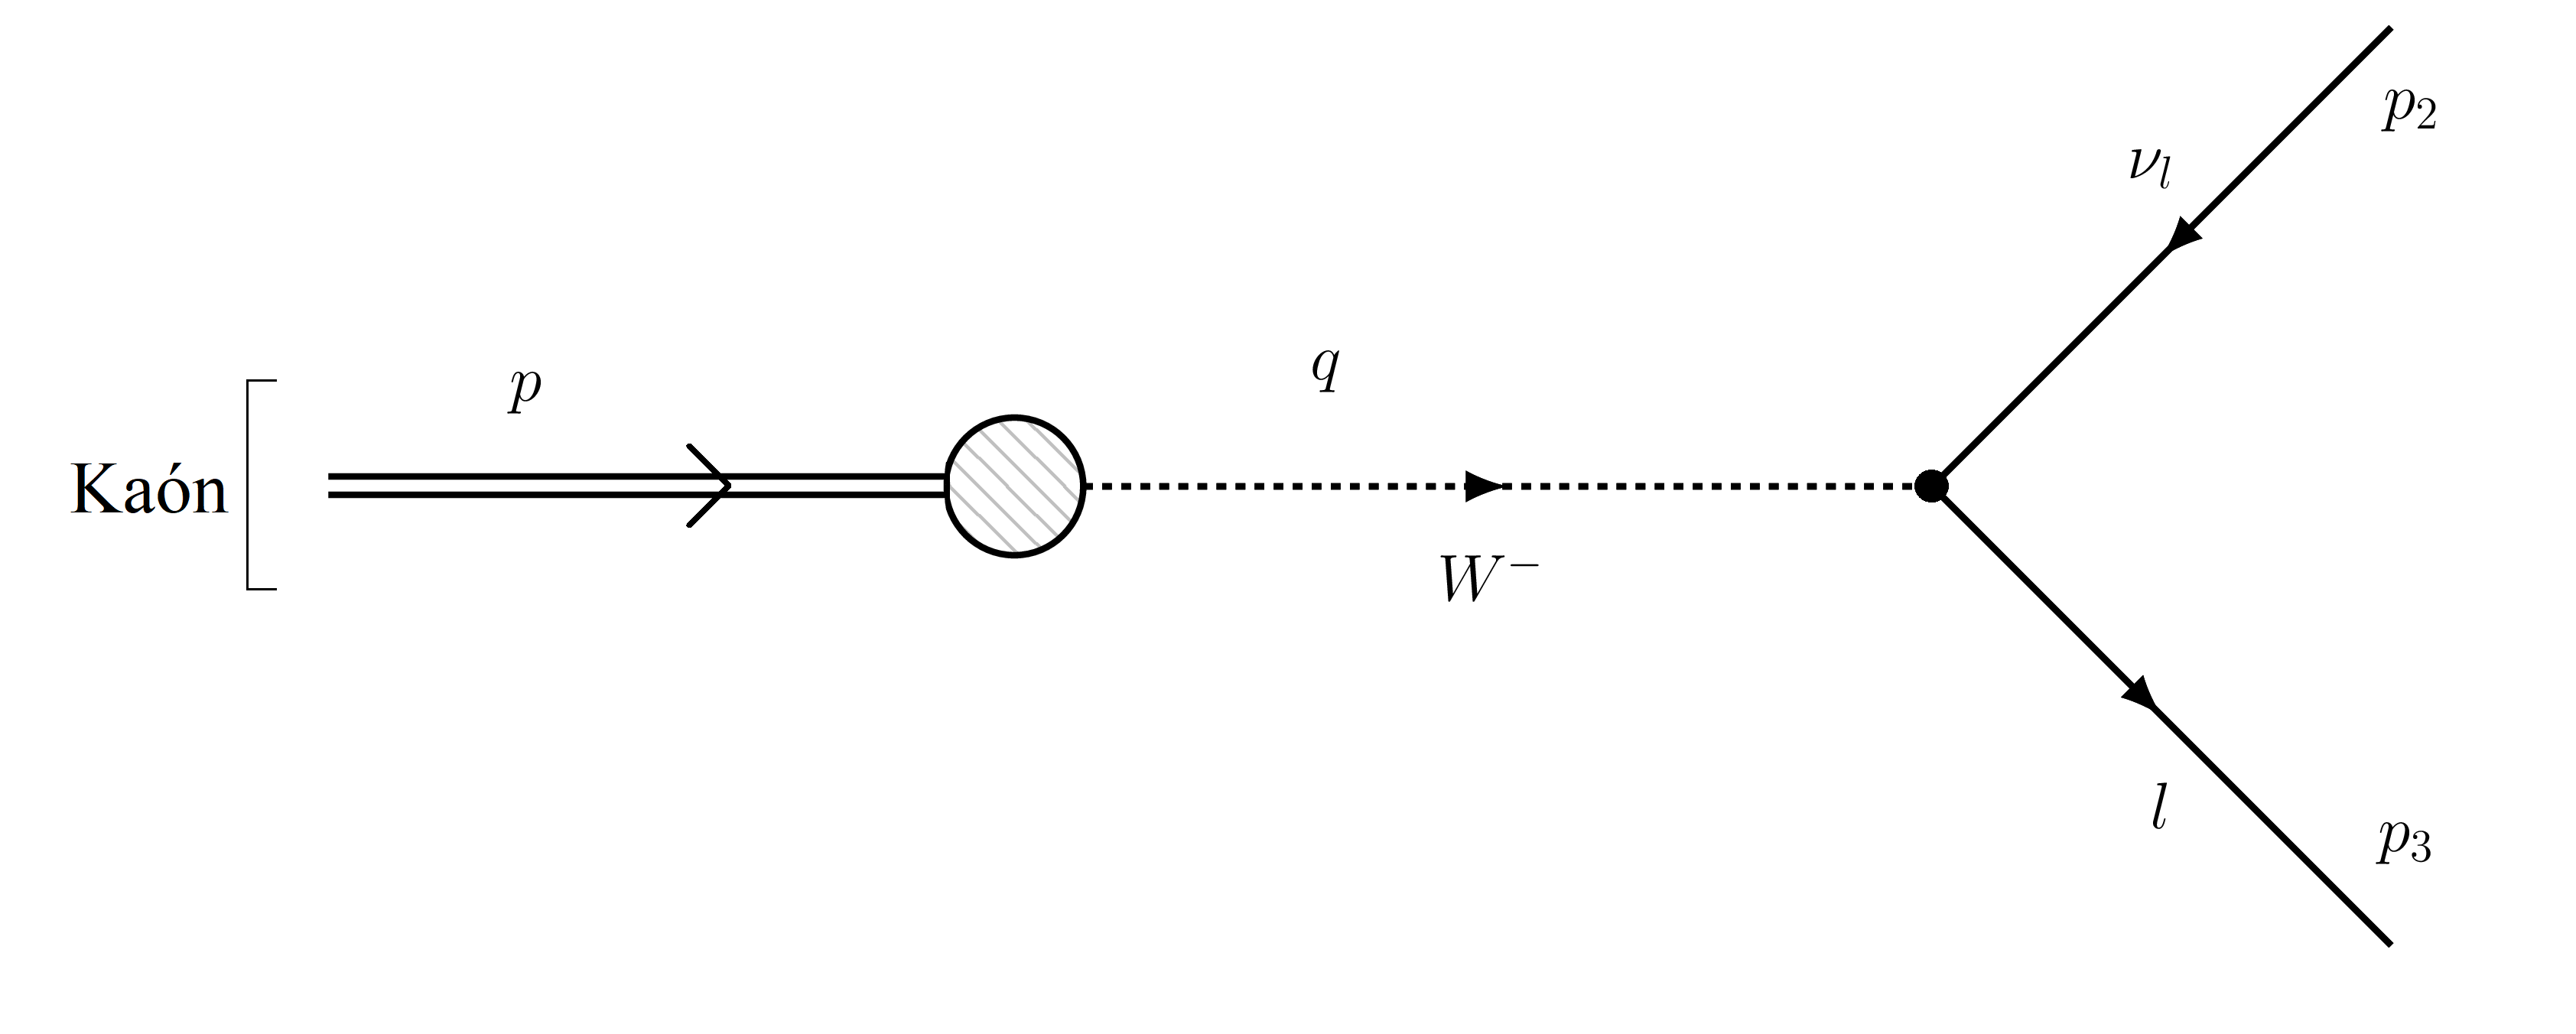
\includegraphics[width=0.95\textwidth]{C:/Users/Carmen/Desktop/Universidad/TFG/Borradores/img/kaon2.png}
	\caption[Diagrama de Feynman de $\PKm \rightarrow \Plm + \Pagnl$ con los momentos]
	{Diagrama de Feynman de $\PKm \rightarrow \Plm + \Pagnl$ con los momentos de cada partícula.}
	\label{fig:diagrama2}
\end{figure}

Analizamos el diagrama de la figura \ref{fig:diagrama2} y aplicamos las reglas de Feynman para calcular la amplitud de decaimiento del proceso, con el objetivo de hallar la probabilidad de que ocurran tales modos de decaimiento. 

Así se obtiene que:
\begin{equation}
\mathcal{M} =\dfrac{{g_{w}}^2}{8\left( M_W\right)^{2}}\left[ \overline{u}\left(3\right) \gamma_{\mu}\left( 1-\gamma^{5} \right) v\left( 2\right) \right] F^{\mu}\label{eq:Msimple}
\end{equation}
con $F^{\mu}=f_K p^{\mu}$, siendo $f_K$ la constante de decaimiento del kaón; desconocida en principio.

Aplicando el truco de Casimir (ver eq. \ref{eq:casimir_trick}) y haciendo la media, se llega a la siguiente expresión:
\begin{equation}
\left\langle |\mathcal{M}|^{2}\right\rangle=\dfrac{1}{8}\left[ f_{K}\left( \dfrac{g_w}{M_W}\right) ^{2}\right] ^{2}\left[2\left( p\cdot p_{2}\right) \left( p\cdot p_{3}\right) -p^{2}\left( p_{2}\cdot p_{3}\right)\right]\label{eq:amplitudM}
\end{equation}

Teniendo en cuenta que $p=p_{2}+p_{3}$ junto con $p^2={m_K}^2$ y ${p_3}^2={m_{\Pl}}^2$, y sabiendo que el antineutrino carece de masa: ${p_2}^2={m_{\nu}}^2=0$, reescribimos:
\begin{align}
p\cdot p_{2} &= p_{3} \cdot p_{2} & p \cdot p_{3} &= p_{2} \cdot p_{3}+{m_{\Pl}}^2
\end{align}

Además,
\begin{equation}
p^{2}={p_{2}}^{2}+{p_3}^{2}+2\left( p_{2} \cdot p_{3}\right) \longrightarrow 2\left( p_{2} \cdot p_{3}\right)=\left( m_{K}^{2}-m_{\Pl}^{2}\right)
\end{equation}

Sustituyendo en la ecuación \ref{eq:amplitudM}, se llega a:
\begin{equation}
\left\langle |\mathcal{M}|^{2}\right\rangle=\left( \dfrac{g_w}{2M_W}\right)^{4} {f_K}^2 {m_{\Pl}}^{2}\left( {m_{K}}^{2}-{m_{\Pl}}^{2}\right)\label{eq:amplitudmedia}
\end{equation}

Así, la expresión final para la probabilidad del decaimiento leptónico de $\PKm$ es:
\begin{equation}
\Gamma =\dfrac{{f_{K}}^{2}}{\pi {m_{K}}^{3}}\left( \dfrac{g_w}{4M_W}\right)^{4}{m_{\Pl}}^{2}\left({m_{K}}^{2}-{m_{\Pl}}^{2}\right)^{2}\label{eq:decayrate}
\end{equation}

Para ver un desarrollo detallado paso a paso de cómo se obtienen las ecuaciones \ref{eq:Msimple}, \ref{eq:amplitudM}, \ref{eq:amplitudmedia} y \ref{eq:decayrate}, consultar el Apéndice \hyperref[cap:B]{B}.

Comparando los dos modos de decaimiento posibles $\PKm \rightarrow \Pem \APnu_{e}$ y $\PKm \rightarrow \Pmuon \APnu_{\mu}$:
\begin{equation}
\dfrac{\Gamma \left( \PKm \rightarrow \Pem \APnu_{e}\right) }{\Gamma \left( \PKm \rightarrow \Pmuon \APnu_{\mu}\right) }=\dfrac{m_{e}^{2}\left( m_{K}^{2}-m_{e}^{2}\right) ^{2}}{m_{\mu }^{2}\left( m_{K}^{2}-m_{\mu }^{2}\right) ^{2}}=\dfrac{\left( 0,511\right) ^{2}\left( 493,677^{2}-0,511^{2}\right) ^{2}}{\left( 105,7\right) ^{2}\left( 493,677^{2}-105,7^{2}\right) ^{2}}=\num{2,57e-5}\label{eq:BRkaon}
\end{equation}

Las masas anteriores tienen unidades de MeV. Si procedemos de forma análoga para el pión $\Pgp$, se tiene que:
\begin{equation}
\dfrac{\Gamma \left( \Pgpm \rightarrow \Pem \APnu_{e}\right) }{\Gamma \left( \Pgpm \rightarrow \Pmuon \APnu_{\mu}\right) }=\dfrac{m_{e}^{2}\left( m_{\pi}^{2}-m_{e}^{2}\right) ^{2}}{m_{\mu }^{2}\left( m_{\pi}^{2}-m_{\mu }^{2}\right) ^{2}}=\dfrac{\left( 0,511\right) ^{2}\left(139,57^{2}-0,511^{2}\right) ^{2}}{\left( 105,7\right) ^{2}\left( 139,57^{2}-105,7^{2}\right) ^{2}}=\num{1,28e-4}\label{eq:BRpion}
\end{equation}

Estos valores de las ratios son muy parecidos a los datos experimentales \cite{tanabashi} \cite{olive}:
\begin{align}
\dfrac{\Gamma \left( \PKm \rightarrow \Pem \APnu_{e}\right)}{\Gamma \left( \PKm \rightarrow \Pmuon \APnu_{\mu}\right)} &= \num{2,488(09)e-5} & \dfrac{\Gamma \left( \Pgpm \rightarrow \Pem \APnu_{e}\right)}{\Gamma \left( \Pgpm \rightarrow \Pmuon \APnu_{\mu}\right)} &= \num{1,230(04)e-4}\label{eq:BRexp}
\end{align}

El resultado de las dos ratios indica que, tanto el pión como el mesón $\PK$, prefieren el modo leptónico del $\Pmuon$ sobre el $\Pem$. En un principio, este hecho puede parecer sorprendente puesto que la masa del muón es mucho mayor que la del electrón y, de acuerdo con las consideraciones de la densidad de estados finales, se favorecen los decaimientos con la disminución de masa más grande. Esto quiere decir que, excluyendo aquellos casos donde intervenga alguna ley de conservación, el estado final de las desintegraciones suele ser el más ligero. 

Los modos leptónicos de $\PK$ y $\Pgp$ suponen una excepción a esta norma. Este hecho puede entenderse teniendo en cuenta que, tanto el pión como el kaón, tienen espín 0, por lo que, para conservar el espín neto nulo y el momento lineal, leptón $\Pl$ y antineutrino $\APnulepton$ deben emitirse con espines opuestos y helicidades iguales. Pero, la interacción débil sólo es sensible a la componente izquierda de la quiralidad, luego el $\APnulepton$ siempre tiene quiralidad izquierda y helicidad positiva ya que, para las antipartículas sin masa, la helicidad es opuesta a la quiralidad. Esto significa que $\Pl$ debe emitirse también con helicidad positiva.

Sin embargo, la helicidad ``correcta'' de los leptones no es la positiva: Si $\Pl$ no tuviera masa, únicamente existiría como una partícula con quiralidad izquierda y helicidad negativa. Más concretamente, si se diera este caso, el $\left( 1-\gamma^{5} \right)$ en el factor del vértice débil se acoplaría sólo a los electrones con quiralidad izquierda, del mismo modo que se acopla sólo a los neutrinos izquierdos. Esto es debido a que en el límite relativista, para partículas sin masa, quiralidad y helicidad coinciden. De esta forma, el modo $\Pem \APnu_{e}$ nunca podría ocurrir. Puesto que este no es el caso y $\Pem$ tiene masa (aunque mucho menor que la del $\Pmuon$), emerge con helicidad positiva para preservar el momento angular. Luego, el modo $\Pem \APnu_{e}$ sí ocurre aunque de forma mucho menos numerosa que el modo $\Pmuon \APnu_{\mu}$ \cite{Griffiths2008} \cite{Halzen}.

Aunque esta justificación parece sugerir que la violación de la paridad en la fuerza débil causa esta supresión del modo electrónico frente al muónico, la razón fundamental radica en la conservación del momento angular y en la estructura vectorial de la interacción débil. Por lo que, incluso una interacción que conserve la paridad produciría la misma supresión, siempre que ésta pueda escribirse en términos de una corriente vector. 

Por ejemplo, si se utiliza el formalismo de la teoría electrodébil, el vértice leptónico se describe entonces mediante un factor $\left( C_{V}-C_{A}\gamma^{5} \right)$, donde $C_{V}$ y $C_{A}$ son constantes reales. Siguiendo el mismo procedimiento, resultaría la misma expresión para la probabilidad de decaimiento salvo un término $\left( {C_{V}}^2+{C_{A}}^2\right)$:
\begin{equation}
\Gamma =\dfrac{{f_{K}}^{2}}{2\pi {m_{K}}^{3}}\left( \dfrac{g_w}{4M_W}\right)^{4}\left( {C_{V}}^2+{C_{A}}^2\right){m_{\Pl}}^{2}\left({m_{K}}^{2}-{m_{\Pl}}^{2}\right)\label{eq:decayrateEWt}
\end{equation}

El caso original se obtendría haciendo $C_{V}=1$ y $C_{A}=-1$. Sin embargo, si hacemos $C_{A}=0$, se mantiene una expresión para $\Gamma$ similar a \ref{eq:decayrate}, y por tanto la misma supresión del modo electrónico. Del mismo modo, si se tiene $C_{V}=0$, también se produce esta supresión. Así, se confirma que la causa responsable de que se prefiera el decaimiento muónico frente al electrónico es la naturaleza vectorial de la corriente débil. Cualquier interacción que presente una estructura de vector, ya sea vector polar, vector axial o una combinación de ambas, produciría la misma preferencia por el modo muónico que tienen $\PK$ y $\Pgp$. Además, que el ratio del mesón $\PK$ \ref{eq:BRkaon} sea un orden de magnitud menor que el del mesón $\Pgp$ \ref{eq:BRpion} se debe a que la masa del kaón $m_{K}$ es bastante mayor que la del pión $m_{\pi}$, suprimiendo aún más el modo leptónico del electrón \cite{Renton}.

Por otra parte, atendiendo al formalismo de la interacción débil en el Modelo de Quarks, se tiene que ahora las constantes de decaimiento $f_{\Pgp}$ y $f_{\PK}$ son prácticamente análogas salvo un factor $\cos \left( \theta _{C}\right)$ y $\sin \left( \theta _{C}\right)$, respectivamente, puesto que el modo leptónico del kaón conlleva un cambio de extrañeza $S$ pero el del pión no. Estudiando el $BR$ del modo leptónico de ambos mesones, se tiene entonces que:
\begin{equation}
BR\left(\PKm / \Pgpm\right)_{\Pl}=\dfrac{\Gamma \left( \PKm \rightarrow \Pl \APnulepton\right) }{\Gamma \left( \Pgpm \rightarrow \Pl \APnulepton\right)}=\tan ^{2}\left( \theta _{C}\right) \left( \dfrac{m_{\pi}}{m_{K}}\right) ^{3}\left( \dfrac{{m_{K}}^{2}-{m_{\Pl}}^{2}}{{m_{\pi}}^{2}-{m_{\Pl}}^{2}}\right) ^{2}
\end{equation}

Sustituyendo el valor de $13,02\degree$ para el ángulo de Cabibbo y las masas correspondientes para el modo electrónico y el muónico, se obtiene $BR\left(\PKm / \Pgpm\right)_{e}=0,19$ y $BR\left(\PKm / \Pgpm\right)_{\mu}=0,96$. Experimentalmente, se ha obtenido que los ratios tienen los valores $BR\left(\PKm / \Pgpm\right)_{e}=0,26$ y $BR\left(\PKm / \Pgpm\right)_{\mu}=1,34$, produciendo en un valor de  $15,4\degree$ para el ángulo de Cabibbo \cite{Griffiths2008}. De los resultados anteriores de los $BR$ se aprecia como $BR\left(\PKm / \Pgpm\right)_{e} \simeq \dfrac{1}{5} BR\left(\PKm / \Pgpm\right)_{\mu}$. 

Asimismo, si tenemos en cuenta las expresiones \ref{eq:meanlife} y \ref{eq:decayrate} junto con los datos empíricos extraídos de \cite{Zyla} para la semivida promedio: $\tau \left(\Pgpm\right)=\SI{2,6033(05)e-8}{\second}$ y $\tau \left(\PKm\right)=\SI{1,2380(20)e-8}{\second}$, se puede calcular el valor numérico de $f_{\Pgp}$ y $f_{\PK}$ \cite{Renton}. 

Considerando el factor de Cabibbo para la corriente hadrónica débil, reescribimos $\Gamma$ para cada mesón como:
\begin{align}
\Gamma\left(\Pgpm \right) =\dfrac{{f_{\pi}}^{2}}{\pi {m_{\pi}}^{3}}\left( \dfrac{g_w}{4M_W}\right)^{4} \cos^{2} \left(\theta_{C}\right)  {m_{\Pl}}^{2}\left({m_{\pi}}^{2}-{m_{\Pl}}^{2}\right)^{2}\label{eq:decayPIcab} \\
\Gamma\left(\PKm \right) =\dfrac{{f_{K}}^{2}}{\pi {m_{K}}^{3}}\left(\dfrac{g_w}{4M_W}\right)^{4} \sin^{2} \left(\theta_{C}\right) {m_{\Pl}}^{2}\left({m_{K}}^{2}-{m_{\Pl}}^{2}\right)^{2}\label{eq:decayKcab}
\end{align}

Sabiendo que $\theta_{C}=13,02\degree$ y $\hbar=\SI{6,582e-16}{\eV\cdot\second}$, despejamos la constante de decaimiento para cada mesón. Además, sustituyendo para el modo muónico las masas de cada partícula $m_{K}=\SI{493,677}{\MeV}$, $m_{\Pl} \equiv m_{\mu}=\SI{105,7}{\MeV}$, $m_{K}=\SI{139,57}{\MeV}$ donde corresponda, se obtiene:
\begin{align}
f_{\Pgp} &= \SI{0,132}{\GeV} \simeq 0,95m_{\pi} & f_{\PK} &= \SI{0,196}{\GeV} \simeq 0,4m_{\PK}
\end{align}

El hecho de que $f_{\Pgp} \approx m_{\pi}$ mientras que $f_{\PK} \simeq 0,4m_{\PK}$  es consecuencia directa del cambio de extrañeza en el decaimiento leptónico del mesón $\PK$. Si $\PKm$ y $\Pgpm$ tuvieran la misma distribución de quarks, $f_{\PK}$ y $f_{\Pgp}$ serían iguales.

Si usáramos la matriz CKM para describir la corriente débil hadrónica, como se hace en el Modelo Estándar, en lugar de la matriz Cabibbo-GIM, reescribiríamos las expresiones \ref{eq:decayPIcab} y \ref{eq:decayKcab} como:
\begin{align}
\Gamma\left(\Pgpm \right) =\dfrac{{f_{\pi}}^{2}|V_{ud}|}{\pi {m_{\pi}}^{3}}\left( \dfrac{g_w}{4M_W}\right)^{4} {m_{\Pl}}^{2}\left({m_{\pi}}^{2}-{m_{\Pl}}^{2}\right)^{2}\label{eq:decayPIckm}\\
\Gamma\left(\PKm \right) =\dfrac{{f_{K}}^{2}|V_{us}|}{\pi {m_{K}}^{3}}\left(\dfrac{g_w}{4M_W}\right)^{4} \sin^{2} {m_{\Pl}}^{2}\left({m_{K}}^{2}-{m_{\Pl}}^{2}\right)^{2}\label{eq:decayKckm}
\end{align}

Entonces, se aprecia que $|V_{ud}|= 0,97370(14) \simeq \cos^{2} \left(\theta_{C}\right)$ y $|V_{us}|= 0,2245(8) \simeq \sin^{2} \left(\theta_{C}\right)$, por lo que los valores calculados anteriormente para $f_{\PK}$ y $f_{\Pgp}$ son muy precisos\protect\footnotemark .

\footnotetext{Valores de $|V_{ud}|$ y $|V_{us}|$ extraídos de \cite{Zyla}.}

\subsubsection{Helicidad y Quiralidad}\label{sec:quirality}
En las expresiones anteriores de la corriente débil aparece el operador $\gamma^5$, que indica la quiralidad de las partículas. A menudo, quiralidad y helicidad son conceptos confundidos. Por este motivo, es conveniente hacer un paréntesis y explicar con detalle en qué consiste cada uno.

La helicidad se define como la proyección del espín de una partícula en la dirección de su momento $\vec{p}$. En el marco teórico de la TCC, la helicidad de la partícula se representa mediante el operador helicidad $\mathcal{H}$:
\begin{equation}
\mathcal{H}=\dfrac{1}{2} \dfrac{\vec{p} \cdot \vec{\sigma}}{p}
\end{equation} 

Para una partícula fermiónica (de espín $1/2$), los autovalores de $\mathcal{H}$ son $+1/2$ (helicidad positiva), si la dirección de su espín coincide con la dirección de su movimiento, y $-1/2$ (helicidad negativa) en el caso contrario \cite{Bettini}. Así pues, los autoestados de helicidad se corresponden a espinores de dos componentes. En general, si la partícula tiene una masa distinta de cero, la helicidad no es un invariante de Lorentz.

La quiralidad es una propiedad de los bi-espinores que se utilizan para definir partículas y se representa por los autoestados del operador $\gamma^5$, con valores propios $\pm 1$. Los estados de quiralidad son designados como positivo o derecha (R) y negativo o izquierda (L), y sus proyectores son:

\begin{align}
\psi_L &= \dfrac{1-\gamma^5}{2}\psi & \psi_R &= \dfrac{1+\gamma^5}{2}\psi
\end{align}

A diferencia de la helicidad, la quiralidad es siempre un invariante de Lorentz. Sin embargo, cuando la partícula fermiónica carece de masa, helicidad y quiralidad coinciden.
El factor $\dfrac{1-\gamma^5}{2}$ es responsable de que la interacción débil presente estructura V-A, provocando a su vez que se viole la conservación de P y C en esta interacción. Todo esto implica que sólo los leptones con quiralidad negativa (izquierda) pueden reaccionar a la fuerza débil.
